%20 min preso!
\documentclass[xcolor=table]{beamer}
\usepackage{beamerthemesplit}
\usepackage{wrapfig}
\usetheme{SPbGU}
\usepackage{pdfpages}
\usepackage{amsmath}
\usepackage{cmap}
\usepackage[T2A]{fontenc}
\usepackage[utf8]{inputenc}
\usepackage[english]{babel}
\usepackage{indentfirst}
\usepackage{amsmath}
\usepackage{tikz}
\usepackage{multirow}
\usepackage[noend]{algpseudocode}
\usepackage{algorithm}
\usepackage{algorithmicx}
\usepackage{fancyvrb}
\usetikzlibrary{calc}
\usetikzlibrary{shapes,arrows}
\usetikzlibrary{arrows,automata}
\usetikzlibrary{positioning}

\usepackage{tabularx}
\newcolumntype{Y}{>{\raggedleft\arraybackslash}X}


\newtheorem{mytheorem}{Theorem}
\renewcommand{\thealgorithm}{}

\newcommand{\tikzmark}[1]{\tikz[overlay,remember picture] \node (#1) {};}
\def\Put(#1,#2)#3{\leavevmode\makebox(0,0){\put(#1,#2){#3}}}

\tikzset{
    state/.style={
           rectangle,
           rounded corners,
           draw=black, very thick,
           minimum height=2em,
           inner sep=2pt,
           text centered,
           },
}

\beamertemplatenavigationsymbolsempty

\title[Граммтики + ИНС]{Формальные граммтики и искусственные нейронные сети для анализа вторичной структуры}
\subtitle[]{Семестровый проект на осень 2019}
% То, что в квадратных скобках, отображается в левом нижнем углу. 
\institute[]{
Лаборатория языковых инструментов JetBrains \\
Санкт-Петербургский государственный университет \\
Математико-механический факультет }

% То, что в квадратных скобках, отображается в левом нижнем углу.
\author[Семён Григорьев]{Семён Григорьев}

\date{14 сентября 2019г.}

\definecolor{orange}{RGB}{179,36,31}

\begin{document}
{
\begin{frame}[fragile]
  \begin{tabular}{p{2.5cm} p{5.5cm} p{2cm}}
   \begin{center}
      
\includegraphics[height=1.5cm]{pictures/jetbrainsResearch.pdf}
    \end{center}
    &
    \begin{center}
      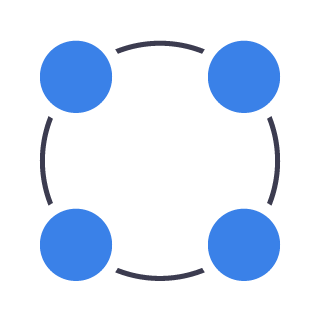
\includegraphics[height=1.5cm]{pictures/bi_logo.png}
    \end{center}
    &
    \begin{center}
      
\includegraphics[height=1.5cm]{pictures/SPbGU_Logo.png}
    \end{center} 
  \end{tabular}
  \titlepage
\end{frame}
}

\begin{frame} \frametitle{Кто мы}
   \begin{itemize}
      \item Исследовательская группа на Математико-Механическом факультете СПбГУ
      \item Исследовательская группа в лаборатории языковых инструментов JetBrains Research
      \item Руководитель группы: Семён Григорьев
      \begin{itemize}
        \item rsdpisuy@gmail.com
        \item semyon.grigorev@jetbrains.com
        \item \url{https://research.jetbrains.org/researchers/gsv}
      \end{itemize}
      \pause
      \item Сферы интереснов
      \begin{itemize}
        \item Теория формальных языков
        \item \textbf{Применение теории формальных языков для решения прикладных задач}
      \end{itemize}
    \end{itemize}
\end{frame}


\begin{frame} \frametitle{Анализ вторичной структуры: синтаксический анализ + искусственные нейронные сети}

\begin{itemize}
  \item Формальная граммтика --- способ описать особенности вторичной структуры 
  \begin{itemize}
     \item А не смоделировать структуру всей цепочки
     \item Используем обыкновенные граммтики, а не вероятностные
  \end{itemize}
  \item Синтаксический анализ --- способ извлечь особенности вторичной структуры
  \item Искусственная нейронная сеть --- вероятностная модель для обработки извлечённых особенностей
\end{itemize}

\end{frame}


\begin{frame}[fragile] \frametitle{Example 3: real tRNA}
\centering

\tikzmark{an}{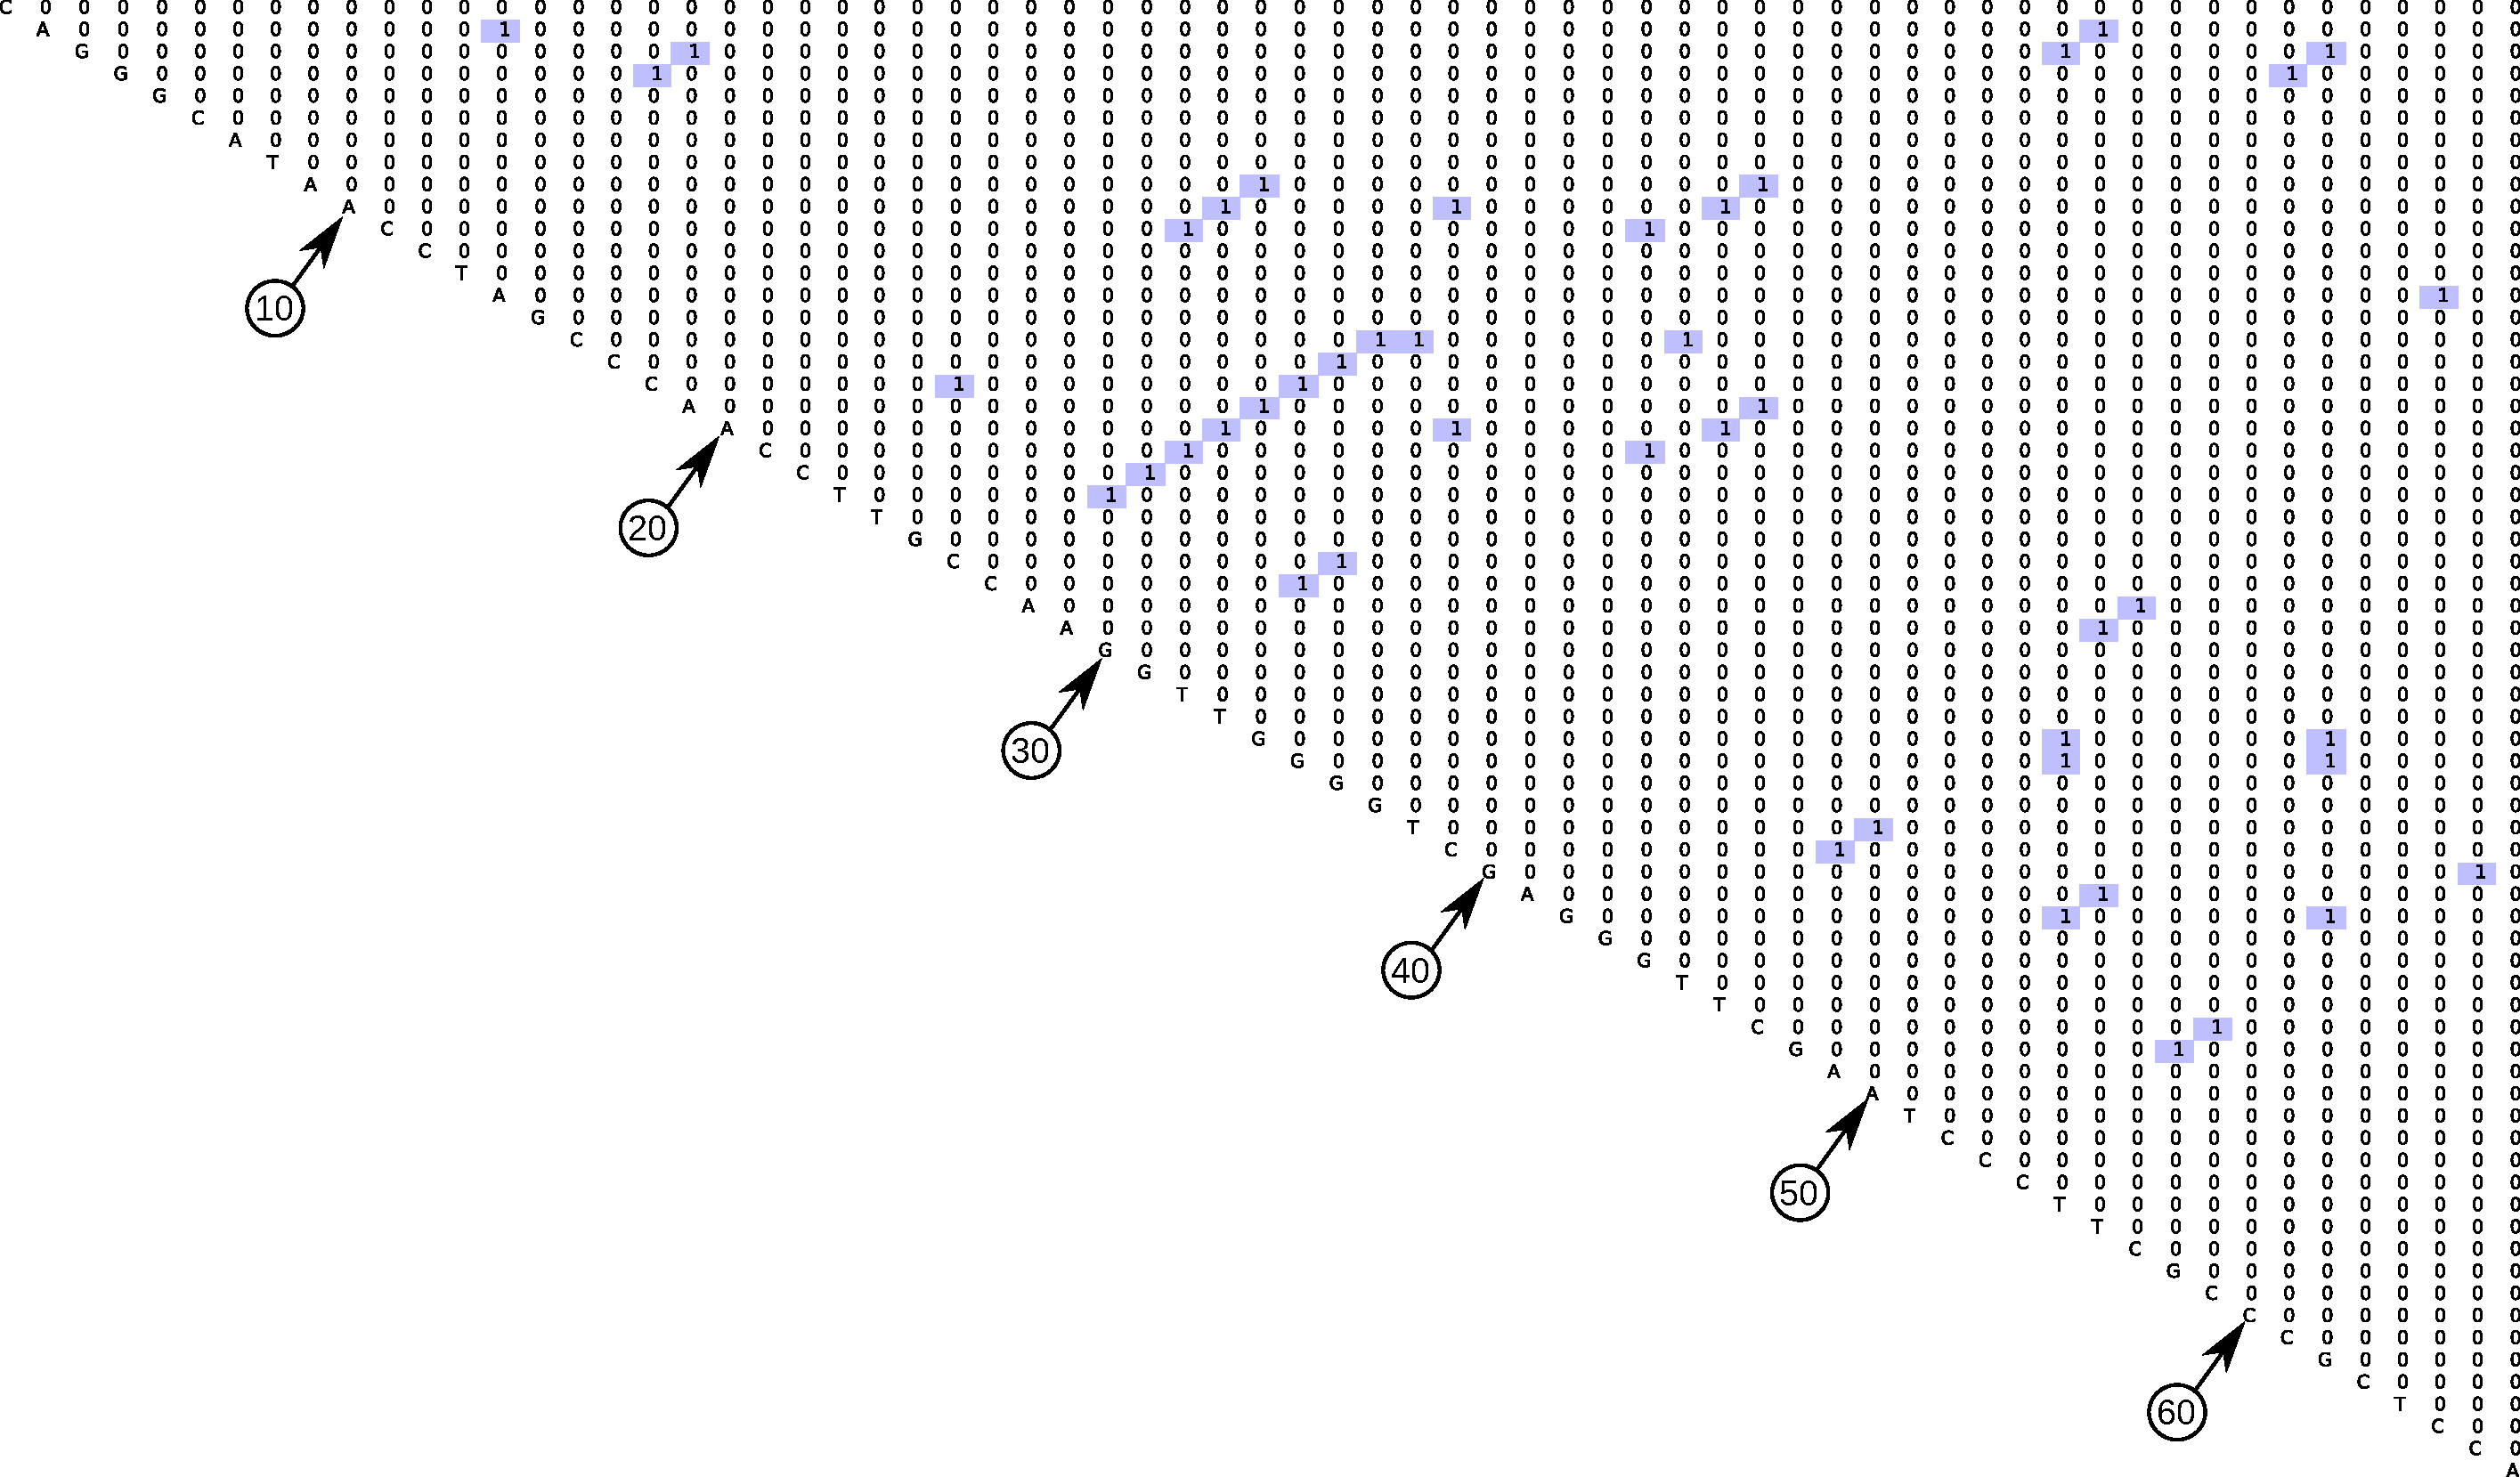
\includegraphics[width=\textwidth]{pictures/0m.pdf}}

\onslide<2-3>{\Put(-175,150){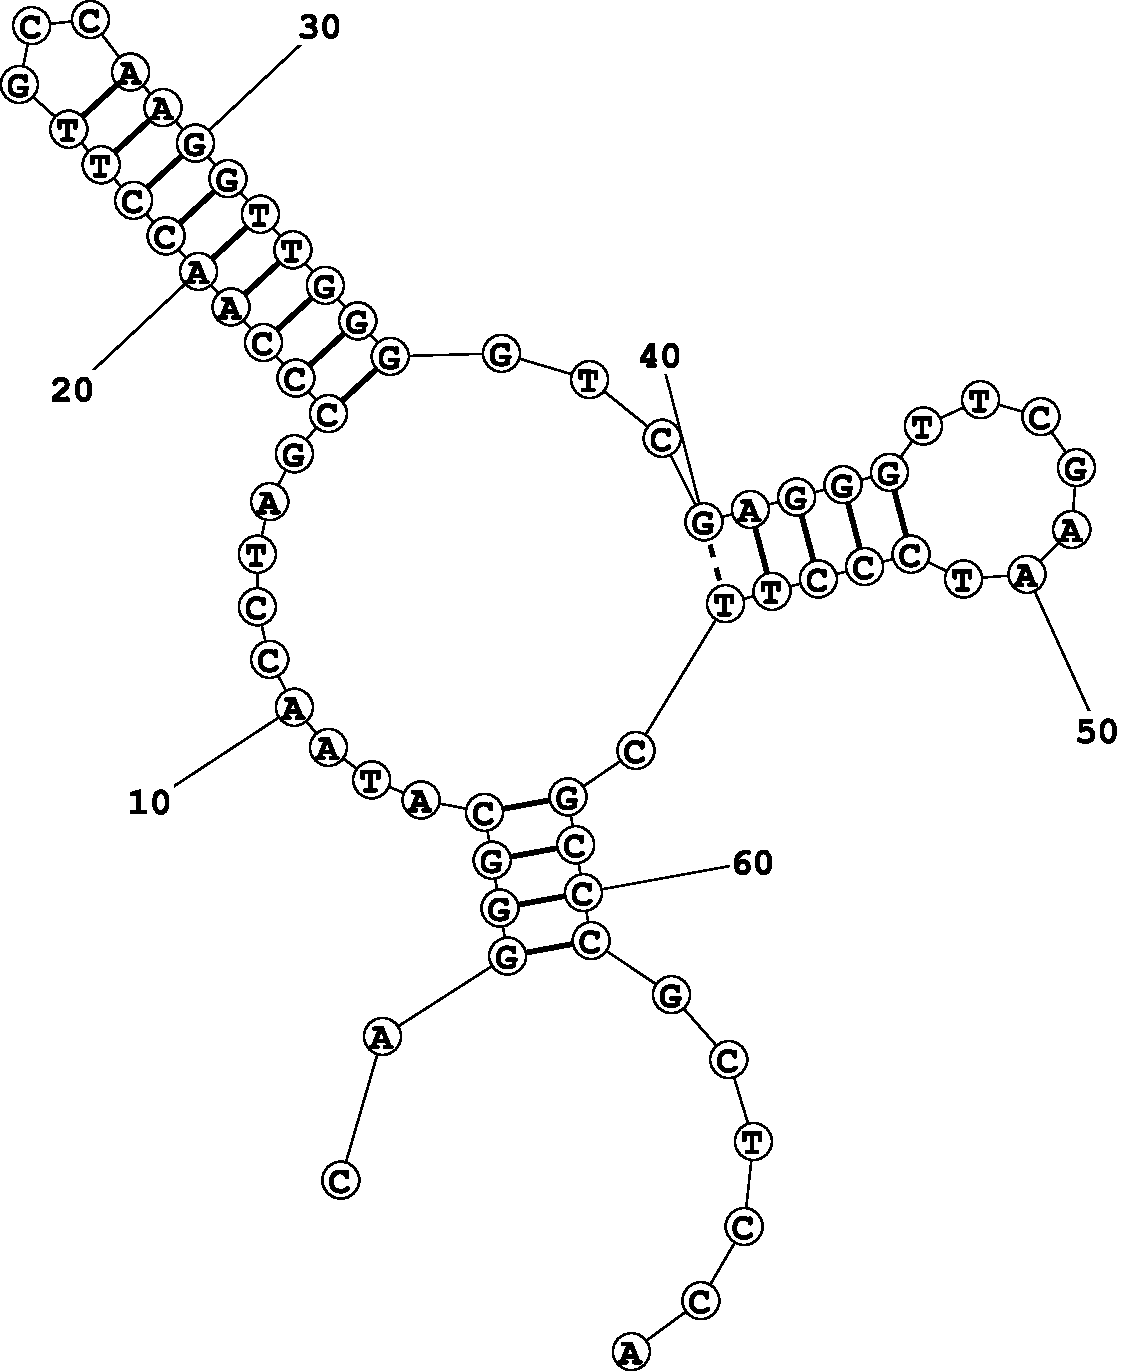
\includegraphics[height=6cm]{pictures/Fold1.pdf}}}
\onslide<3-3>{
\tikz[overlay,remember picture]{
\draw[draw=blue,thick,fill opacity=0.2] ($(an) + (0.28,6.885)$) rectangle ($(an) + (11.22,6.415)$);
\draw[draw=blue,thick,fill opacity=0.2] ($(an) + (10.3,6.885)$) rectangle ($(an) + (11.025,0.57)$);

\draw[draw=blue,thick,fill opacity=0.2] ($(an) + (2.65,5.49)$) rectangle ($(an) + (6.68,4.42)$);
\draw[draw=blue,thick,fill opacity=0.2] ($(an) + (4.65,5.49)$) rectangle ($(an) + (6.46,3.2)$);

\draw[draw=blue,thick,fill opacity=0.2] ($(an) + (7.2,2.85)$) rectangle ($(an) + (10.12,2.4)$);
\draw[draw=blue,thick,fill opacity=0.2] ($(an) + (9.23,2.85)$) rectangle ($(an) + (9.95,1.2)$);
}
}


\end{frame}



\begin{frame} \frametitle{Задачи}
   \begin{itemize}
      \item Подготовка данных для обучения нейронных сетей
      \begin{itemize}
        \item Поиск и анализ баз РНК-цепочек
        \item Подготовка набора данных для обучения: фильтрация, сбор метаданных, приведение к общему формату
      \end{itemize}
      \pause
      \item Подготовка инструментария для анализа вторичной структуры
      \begin{itemize}
        \item Анализ и сравнение существующих инструментов предсказания вторичной структуры РНК последовательностей
        \item Выбор лучшего и его интеграция в процесс обучения нейронных сетей
      \end{itemize}
    \end{itemize}
\end{frame}

\begin{frame} \frametitle{Требования к кандидатам}
   \begin{itemize}
      \item Знание Python (потребуется для автоматизации процесса)
      \item Знание C/C++ и сопутствующего инструментария (потребуется при работе с интсрументами анализа вторичной структуры)
    \end{itemize}
\end{frame}


\begin{frame} \frametitle{Перспективы развития}
   \begin{itemize}
      \item Создание и обучение моделей для различных задач: предсказание вторичной структуры, классификация, фильтрация химер
      \item Применить аналогичный подход к белковым цепочкам
      \item Курсовая/диплом/публикация
    \end{itemize}
\end{frame}



\begin{frame}[fragile] \frametitle{Грамматика}
\begin{verbatim}
s1: stem<s0>
any_str: any_smb*[2..10]
any_smb: A | T | C | G
stem1<s>:               \\ stem of height exactly 1
      A s T | T s A | C s G | G s C
stem3<s>:               \\ stem of height exactly 3
      stem1< stem1< stem1<s> > >
stem<s>:                \\ stem of height 3 or more
      A stem<s> T
    | T stem<s> A
    | C stem<s> G
    | G stem<s> C
    | stem3<s>
s0: any_str | any_str stem<s0> s0
\end{verbatim}
\tikzmark{yyy}{
}
%}
\pause
\onslide<2>{\tikz[overlay,remember picture]{\draw[draw=red,thick,double,fill opacity=0.2] ($ (yyy) + (-0.2,7.5)$) rectangle ($ (yyy) + (12,7)$);}}
\onslide<3>{\tikz[overlay,remember picture]{\draw[draw=red,thick,double,fill opacity=0.2] ($ (yyy) + (-0.2,7)$) rectangle ($ (yyy) + (12,6)$);}}
\onslide<4>{\tikz[overlay,remember picture]{\draw[draw=red,thick,double,fill opacity=0.2] ($ (yyy) + (-0.2,6)$) rectangle ($ (yyy) + (12,5.1)$);}}
\onslide<5>{\tikz[overlay,remember picture]{\draw[draw=red,thick,double,fill opacity=0.2] ($ (yyy) + (-0.2,5.1)$) rectangle ($ (yyy) + (12,4.1)$);}}
\onslide<6>{\tikz[overlay,remember picture]{\draw[draw=red,thick,double,fill opacity=0.2] ($ (yyy) + (-0.2,4.1)$) rectangle ($ (yyy) + (12,1.2)$);}}
\onslide<7>{\tikz[overlay,remember picture]{\draw[draw=red,thick,double,fill opacity=0.2] ($ (yyy) + (-0.2,1.2)$) rectangle ($ (yyy) + (12,0.7)$);}}
\end{frame}


\begin{frame}[fragile] \frametitle{Пример 1: Stem}
\centering
 \texttt{CCCC{\color{red}ATTGCCAAGG}ACCCCA{\color{red}CCTTGGCAAT}CCC}
\vspace{1cm}

\tikzmark{xx}{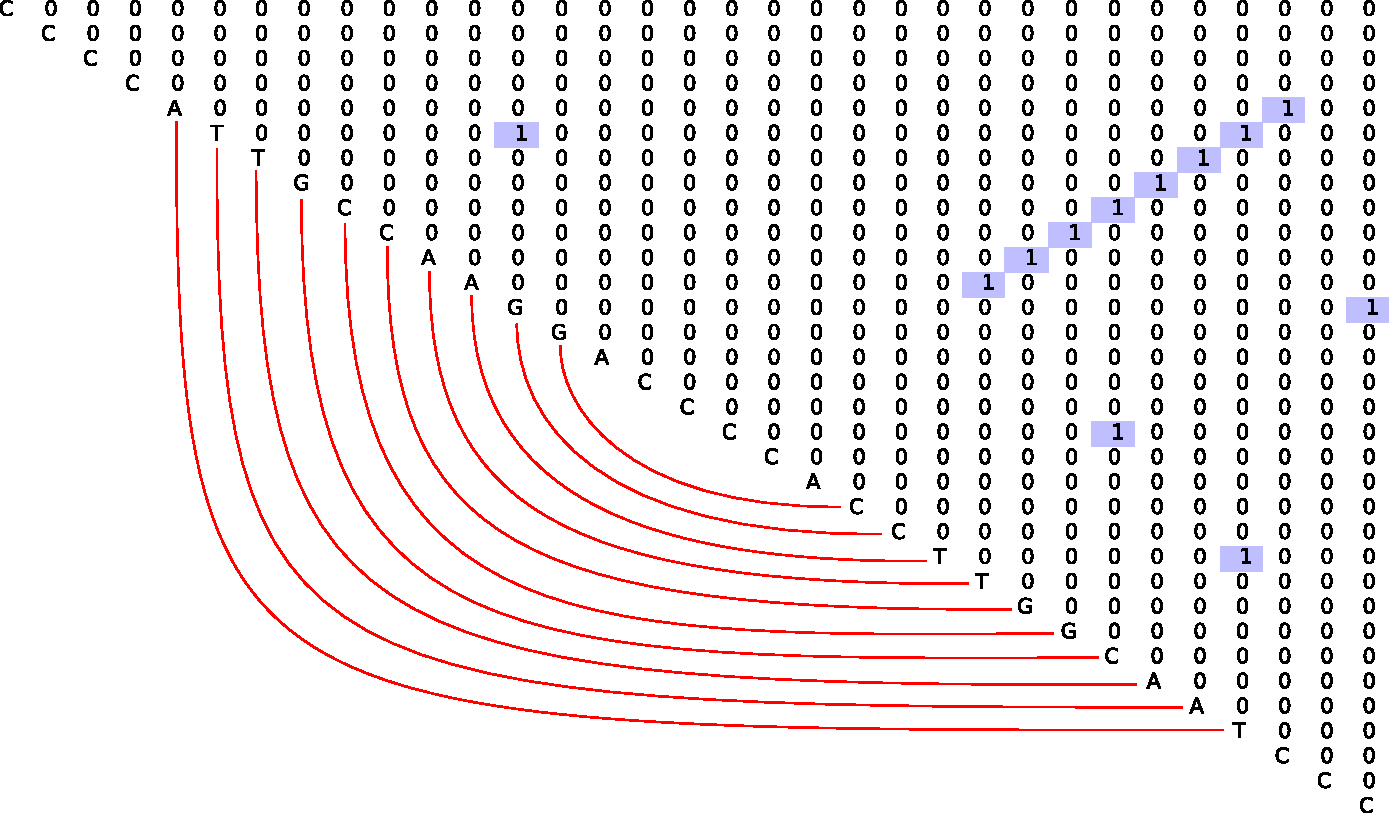
\includegraphics[width=.8\textwidth]{pictures/4.pdf}}
\onslide<2-3>{
\tikz[overlay,remember picture]{
\draw[draw=red,thick,fill opacity=0.2] ($(xx) + (1.1,4.97)$) rectangle ($(xx) + (9.05,3.235)$);
}
}

\onslide<3>{
\tikz[overlay,remember picture]{
\draw[draw=red,thick,fill opacity=0.2] ($(xx) + (5.8,4.97)$) rectangle ($(xx) + (8.75,0.4)$);
}
}

\end{frame}

\begin{frame}[fragile] \frametitle{Пример 2: псевдоузел}
\centering
 \texttt{CC{\color{red}ACTTA}CC{\color{blue}TATGA}CC{\color{red}TAAGT}CC{\color{blue}TCATA}CC}
\vspace{1cm}

\tikzmark{y}{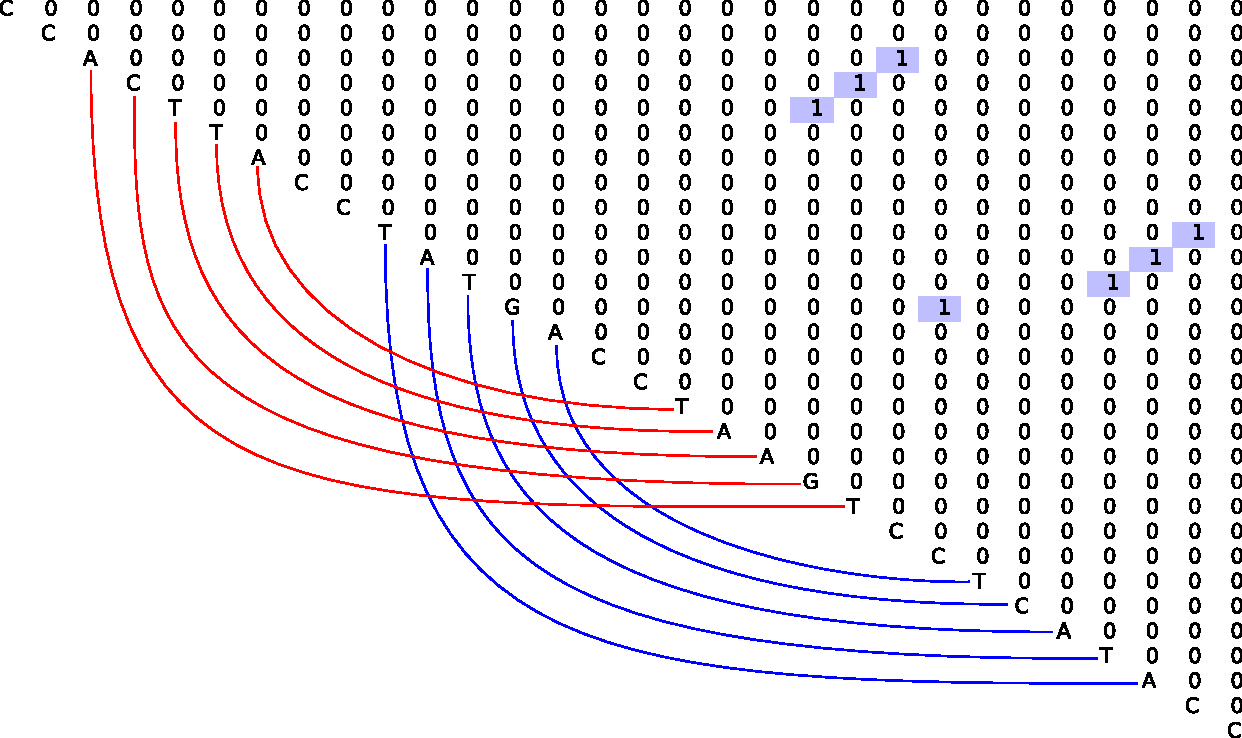
\includegraphics[width=.8\textwidth]{pictures/5.pdf}}

\onslide<2-3>{
\tikz[overlay,remember picture]{
\draw[draw=red,thick,fill opacity=0.2] ($(y) + (0.6,5.37)$) rectangle ($(y) + (7.15,4.4)$);
\draw[draw=red,thick,fill opacity=0.2] ($(y) + (5.15,5.37)$) rectangle ($(y) + (6.8,1.7)$);
}
}

\onslide<3>{
\tikz[overlay,remember picture]{
\draw[draw=blue,thick,fill opacity=0.2] ($(y) + (2.8,4.01)$) rectangle ($(y) + (9.42,3.05)$);
\draw[draw=blue,thick,fill opacity=0.2] ($(y) + (7.45,4.01)$) rectangle ($(y) + (9.1,0.3)$);
}
}

\end{frame}

\begin{frame}[fragile] \frametitle{Example 3: real tRNA}
\centering
 \texttt{CAGGGCATAACCTAGCCCAACCTTGCCAAGG\\TTGGGGTCGAGGGTTCGAATCCCTTCGCCCGCTCCA}
\vspace{0.5cm}
\begin{itemize}
  \item Novosphingobium aromaticivorans DSM 12444 chr.trna57-GlyGCC(268150-268084) Gly (GCC) 67 bp Sc: 22.9, from \href{http://gtrnadb2009.ucsc.edu/download.html}{GtRNAdb}
  \item Predicted secondary structures are given by using the \href{http://rna.urmc.rochester.edu/RNAstructureWeb/Servers/Fold/Fold.html}{Fold Web Server with default settings}

\end{itemize}
\end{frame}


\begin{frame}[fragile] \frametitle{Example 3: real tRNA}
\centering

\tikzmark{an}{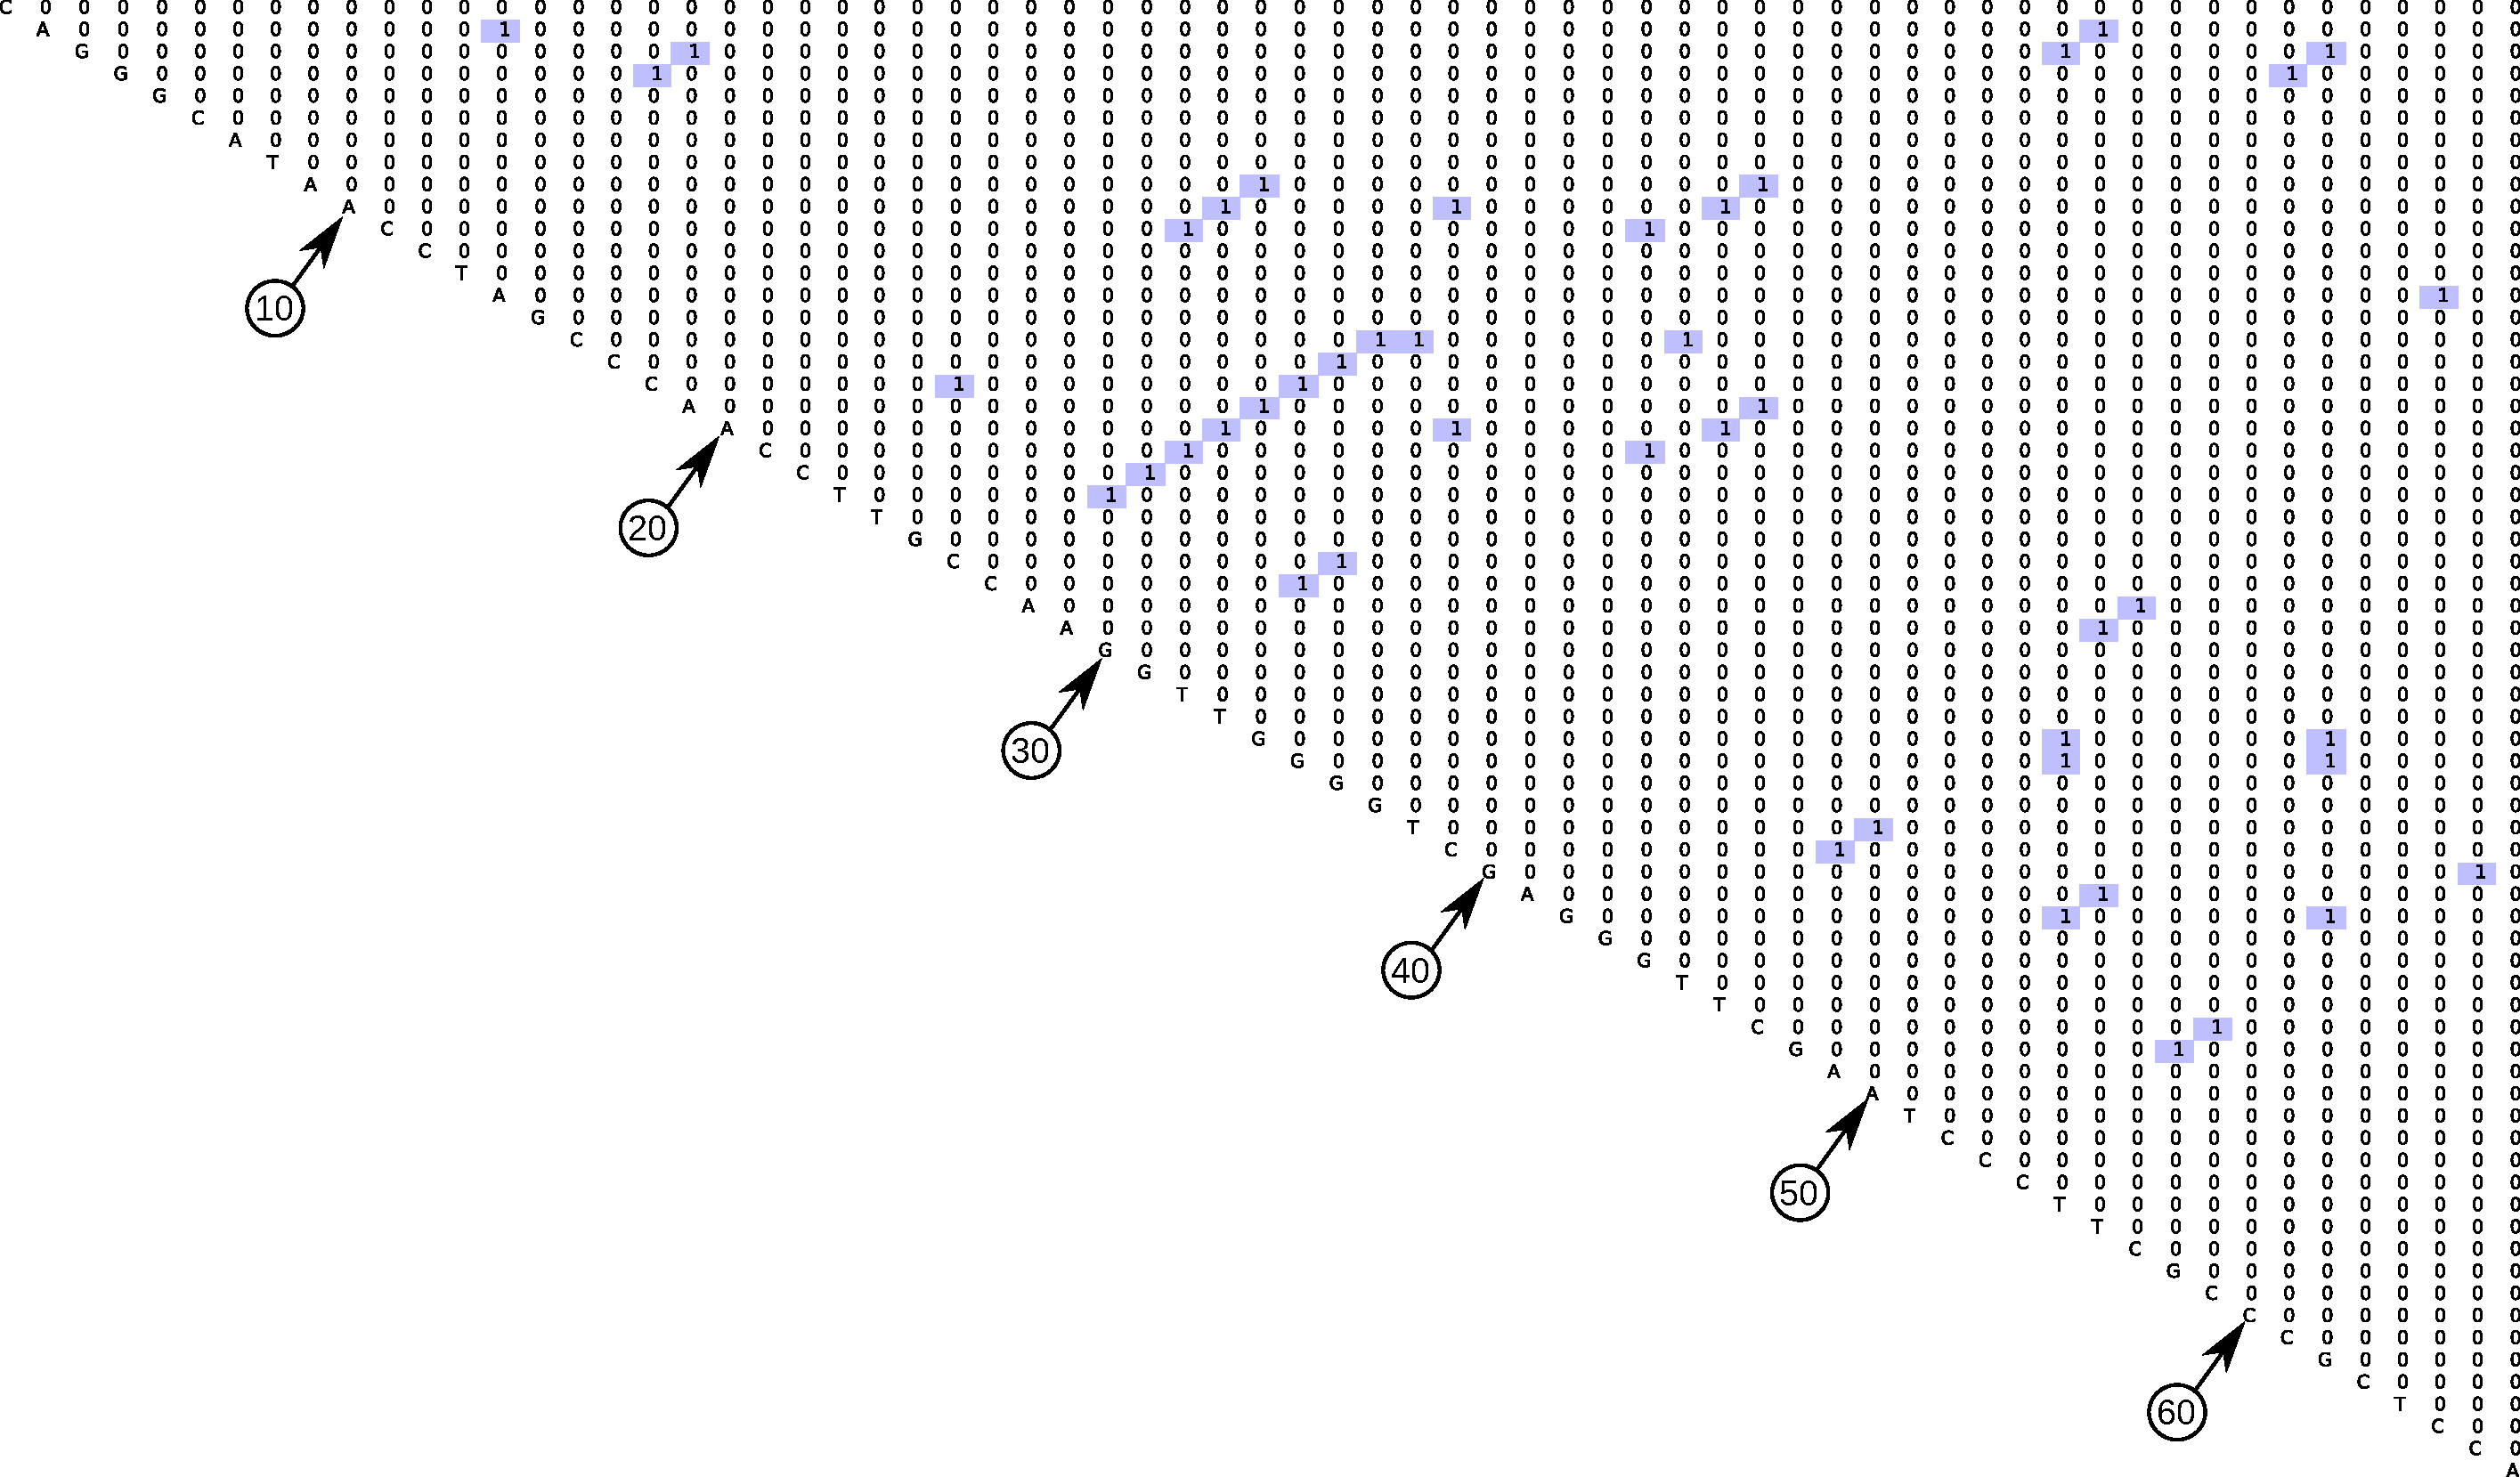
\includegraphics[width=\textwidth]{pictures/0m.pdf}}

\onslide<2-3>{\Put(-175,150){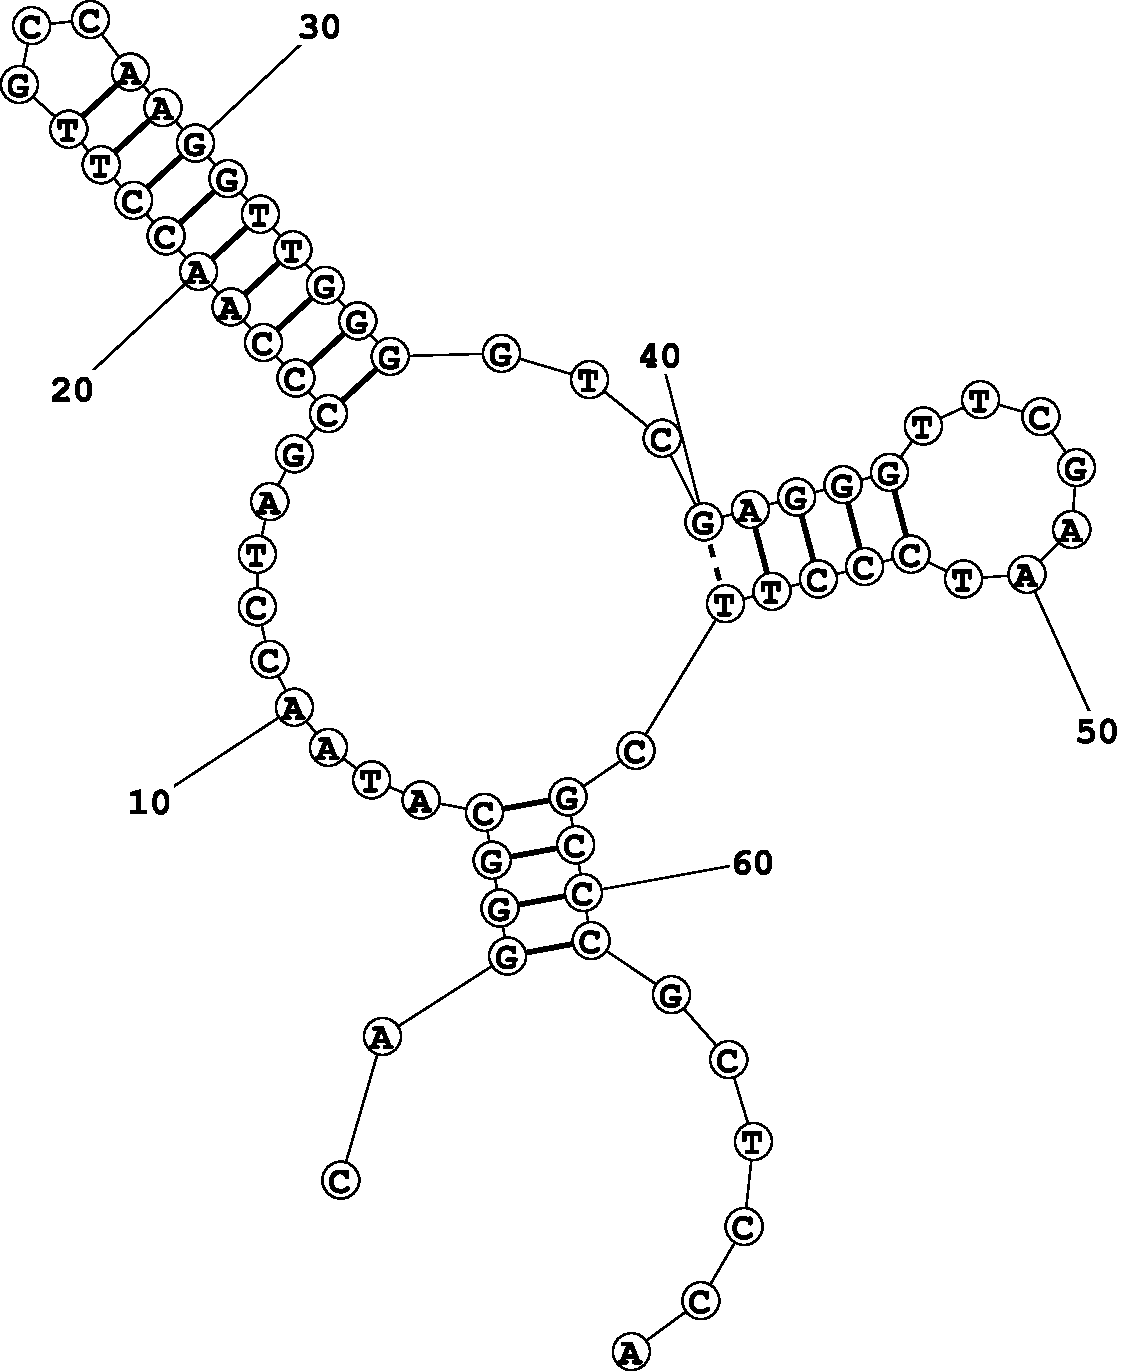
\includegraphics[height=6cm]{pictures/Fold1.pdf}}}
\onslide<3-3,7>{
\tikz[overlay,remember picture]{
\draw[draw=blue,thick,fill opacity=0.2] ($(an) + (0.28,6.885)$) rectangle ($(an) + (11.22,6.415)$);
\draw[draw=blue,thick,fill opacity=0.2] ($(an) + (10.3,6.885)$) rectangle ($(an) + (11.025,0.57)$);

\draw[draw=blue,thick,fill opacity=0.2] ($(an) + (2.65,5.49)$) rectangle ($(an) + (6.68,4.42)$);
\draw[draw=blue,thick,fill opacity=0.2] ($(an) + (4.65,5.49)$) rectangle ($(an) + (6.46,3.2)$);

\draw[draw=blue,thick,fill opacity=0.2] ($(an) + (7.2,2.85)$) rectangle ($(an) + (10.12,2.4)$);
\draw[draw=blue,thick,fill opacity=0.2] ($(an) + (9.23,2.85)$) rectangle ($(an) + (9.95,1.2)$);
}
}

\onslide<5-6>{\Put(-10,130){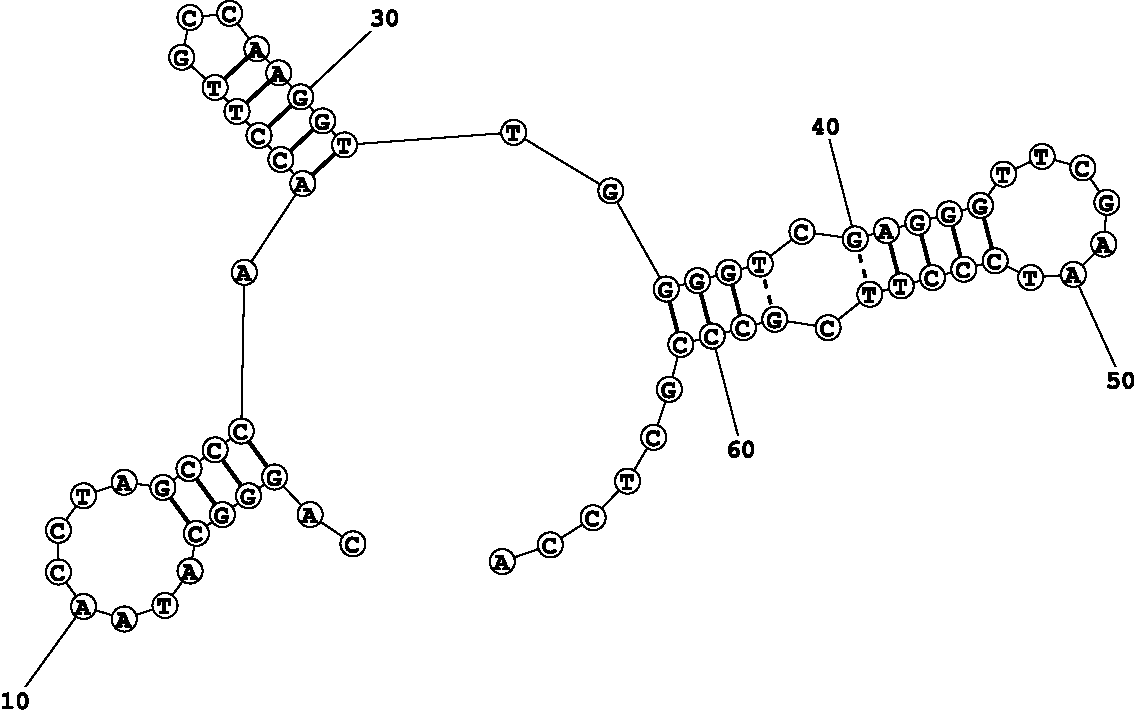
\includegraphics[height=4.3cm]{pictures/Fold2.pdf}}}
\onslide<6-7>{
\tikz[overlay,remember picture]{

\draw[draw=red,thick,fill opacity=0.2] ($(an) + (0.31,6.86)$) rectangle ($(an) + (3.4,6.44)$);
\draw[draw=red,thick,fill opacity=0.2] ($(an) + (2.5,6.86)$) rectangle ($(an) + (3.2,5.1)$);

\draw[draw=red,thick,fill opacity=0.2] ($(an) + (3.4,5.06)$) rectangle ($(an) + (5.95,4.535)$);
\draw[draw=red,thick,fill opacity=0.2] ($(an) + (4.83,5.06)$) rectangle ($(an) + (5.73,3.6)$);

\draw[draw=red,thick,fill opacity=0.2] ($(an) + (6.1,3.47)$) rectangle ($(an) + (11.2,3.15)$);
\draw[draw=red,thick,fill opacity=0.2] ($(an) + (10.5,3.47)$) rectangle ($(an) + (11,0.6)$);

\draw[draw=red,thick,fill opacity=0.2] ($(an) + (7.2,2.85)$) rectangle ($(an) + (10.12,2.4)$);
\draw[draw=red,thick,fill opacity=0.2] ($(an) + (9.23,2.85)$) rectangle ($(an) + (9.95,1.2)$);
}
}
\end{frame}

\begin{frame} \frametitle{Solution Structure}
\tiny %\hspace{-2cm}
  \begin{tikzpicture}[->,>=stealth']


  \node[state,
        align=left,
        text width = 3.5cm] (grm)
   {
    \textbf{Grammar}\\
  Fixed formal grammar (not necessarily context-free) describes features of secondary structure and can be tuned to increase the quality of result.

   };


  \node[state,
        below of=grm,
        node distance=1.5cm,
        align = left,
        text width = 3.5cm] (sqs)
   {
   \textbf{Sequences}\\
  Each sequence is treated as a text in $\{A, C, G, T\}$ alphabet.
   };


  \node[state,
        right of=grm,
        node distance=4cm,
        align = left,
        text width = 3.5cm](parser)
  {
  \textbf{Parser}\\
  Parser extracts features of the given sequence secondary structure.
  Implementation of parsing algorithm is based on matrix multiplications (Valiant, Okhotin) and utilizes GPGPU.
  };

  \node[state,
        right of=parser,
        node distance=4cm,
        align = left,
        text width = 3.5cm] (mtrx)
  {
    \textbf{Matrices}\\
    %\vspace{0.05cm}
    \[ \left( \begin{array}{cccc}
    0 & \textbf{1} & 0 & \textbf{1}\\
    0 & 0 & \textbf{1} & 0\\
    0 & 0 & 0 & \textbf{1}\\
    0 & 0 & 0 & 0
    \end{array} \right)\]
    \vspace{-0.1cm}

  Parsing result is (0-1) matrix~$M$ which represents secondary structure features for sequence $\omega$: $ M[i,j] = 1 \iff \text{\ttfamily{s1}} \xrightarrow{*}{} \omega[i,j]$, and $0$ otherwise.
  };

  \node[state,
        below of=sqs,
        node distance=1cm,
        align = left,
        text width = 3.5cm](result)
  {
  \textbf{Result of classification}

  };


  \node[state,
        below of=parser,
        node distance=4.2cm,
        align = left,
        text width = 3.5cm](DNN)
  {
  \textbf{Neural Network}\\

  Dense neural network with more than 10 dense layers.
  Agressive dropout and batch normalization for learning process stabilization.\\
  Typical building block:
  \\
  \vspace{-0.3cm}
  \begin{center}
  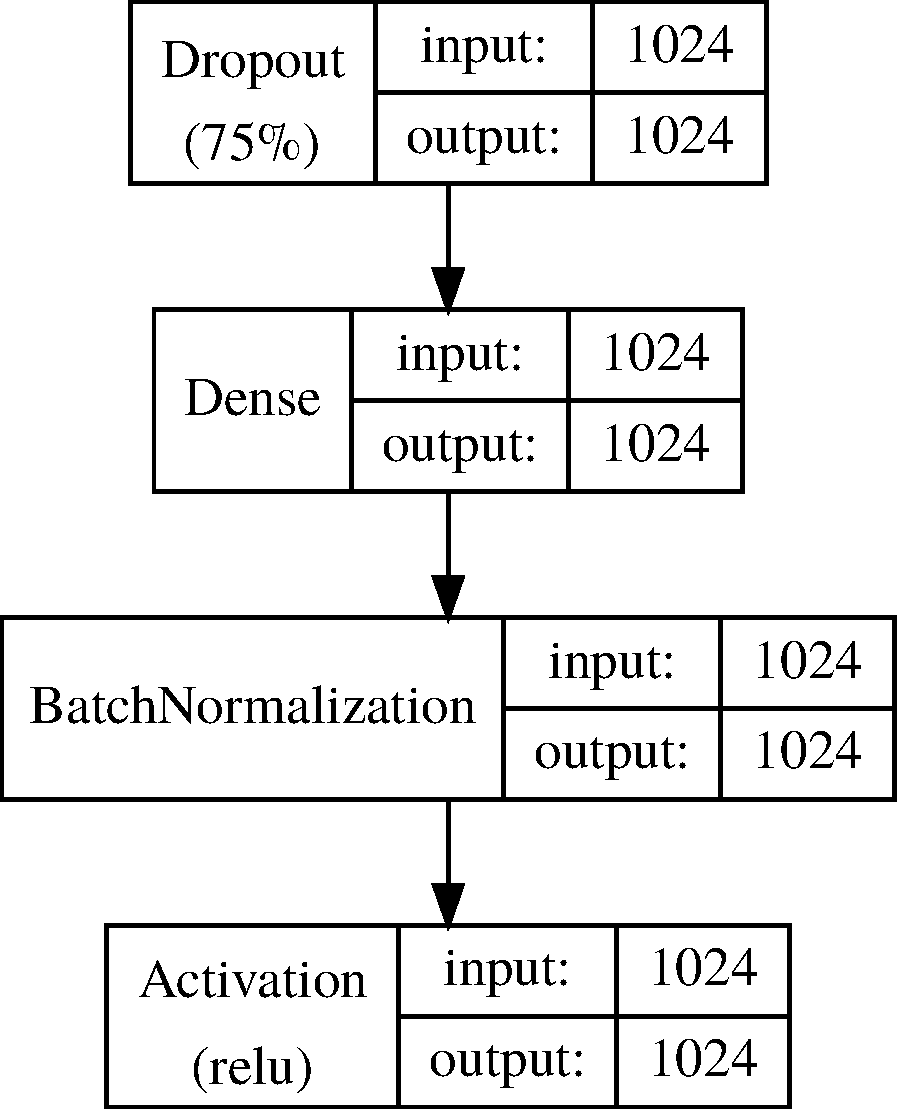
\includegraphics[width=2.5cm]{pictures/bb.pdf}
  \end{center}

  };


  \node[state,
        right of=DNN,
        node distance=4cm,
        align = left,
        text width = 3.5cm](vector)
  {
  \textbf{Vectors}\\
  \vspace{-0.1cm}

\[ \left( \begin{array}{cccc}
0 & 1 & 0 & 1\\
0 & 0 & 1 & 0\\
0 & 0 & 0 & 1\\
0 & 0 & 0 & 0
\end{array} \right) \]
\vspace{-0.35cm}
$$\Downarrow$$
\vspace{-0.35cm}
$$\texttt{[0,1,0,1,0,1,0,0,1,0]}$$
\vspace{-0.35cm}
$$\Downarrow$$
\vspace{-0.35cm}
$$\texttt{[84,128]}$$
%\vspace{-0.1cm}
  Line-by-line compressed matrix representation: sequence of 8 cells (bits) is compressed into a byte. Bottom left triangle of the matrix is always empty, so can be ignored.
  };


  \path (grm) edge  (parser)
   (sqs) edge [bend right] (parser)
  % (sqs) edge (parser)
   (parser) edge (mtrx)
   (mtrx) edge (vector)
   (vector) edge (DNN)
   (DNN) edge (result)
   ;

  \end{tikzpicture}

  \tikzmark{zzz}{
  }
  %}
  \pause
  \onslide<2>{\tikz[overlay,remember picture]{\draw[draw=red,thick,double,fill opacity=0.2] ($ (zzz) + (-0.1,7.9)$) rectangle ($ (zzz) + (3.8,4.8)$);}}

  \onslide<3>{\tikz[overlay,remember picture]{\draw[draw=red,thick,double,fill opacity=0.2] ($ (zzz) + (3.8,7.9)$) rectangle ($ (zzz) + (7.8,5.9)$);}}

  \onslide<4>{\tikz[overlay,remember picture]{\draw[draw=red,thick,double,fill opacity=0.2] ($ (zzz) + (7.8,8.5)$) rectangle ($ (zzz) + (11.8,5.25)$);}}

  \onslide<5>{\tikz[overlay,remember picture]{\draw[draw=red,thick,double,fill opacity=0.2] ($ (zzz) + (7.8,5.1)$) rectangle ($ (zzz) + (11.8,0.35)$);}}

  \onslide<6>{\tikz[overlay,remember picture]{\draw[draw=red,thick,double,fill opacity=0.2] ($ (zzz) + (3.9,5.2)$) rectangle ($ (zzz) + (7.8,0.2)$);}}

  \onslide<7>{\tikz[overlay,remember picture]{\draw[draw=red,thick,double,fill opacity=0.2] ($ (zzz) + (-0.1,4.8)$) rectangle ($ (zzz) + (3.8,4.0)$);}}


\end{frame}


\end{document}
